\cleartooddpage[\thispagestyle{empty}]
\chapter{Tabular Data Structure}\label{tbl}
\moduleinfo{tbl}
The ``tbl'' module implements an object-oriented tabular datatype in Tcl. 
This datatype is suitable for row-oriented two-dimensional data, and efficiently handles sparse tables. 

This is achieved internally by representing the table by five properties: ``keyname'', ``fieldname'', ``keys'', ``fields'', and ``data''. The property ``keyname'' describes what the table keys represent, and the property ``fieldname'' describes what the table fields represent (this is not typically present in raw table formats such as CSV). The property ``keys'' is an ordered list of all the row names of the table, and the property ``fields'' is an ordered list of all the field names of the table. The property ``data'' stores the table values in an unordered nested dictionary, with the first level data keys corresponding to the table keys, and the second level data keys corresponding to the table fields. The conceptual layout of the five properties of a table is illustrated in the figure below.
\vspace{\baselineskip}
\FloatBarrier
\begin{figure}[!htb]
    \centering
    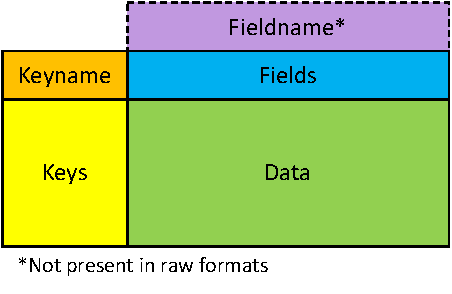
\includegraphics{table}
    \caption{The five properties of a table}
    \label{fig:table_props}
\end{figure}
\clearpage
\section{Creating Table Objects}
Table objects are created from the \cmdlink{tdatbl} class using the standard methods \textit{new} or \textit{create}. 
Once created, table objects act as commands with an ensemble of subcommands, or methods. 
These objects can be copied with the method \methodlink[0]{tdatbl}{copy} and deleted with the method \methodlink[0]{tdatbl}{destroy}.
\begin{syntax}
\command{tdatbl} new \$arg1 \$arg2 ...\\
tdatbl create \$objectName \$arg1 \$arg2 ...
\end{syntax}
\begin{args}
\$objectName & Explicit name for object. \\
\$arg1 \$arg2 ... & Arguments to pass to \methodlink[0]{tdatbl}{define} method.
\end{args}

\begin{example}{Creating a table object}
\begin{lstlisting}
set tableObj [table new]
\end{lstlisting}
\end{example}
\subsection{Copying Table Objects}
The method \methodlink[0]{tdatbl}{copy} copies all the data from a table object to a new object.
\begin{syntax}
\method{tdatbl}{copy} <\$objectName>
\end{syntax}
\begin{args}
\$objectName & Explicit name for object. By default, returns an auto-generated name.
\end{args}

\subsection{Removing Table Objects}
The standard method \methodlink[0]{tdatbl}{destroy} removes a table object from the interpreter. 
\begin{syntax}
\method{tdatbl}{destroy}
\end{syntax}
\clearpage
\section{Table Definition}
The method \methodlink[0]{tdatbl}{define} sets the property values of a table, filtering the data or adding keys and fields as necessary. For example, if the keys are defined to be a subset of the current fields, it will filter the data to only include the key subset. 
Also, if the data is defined, all existing data will be wiped, and any new keys or fields will be added.
\begin{syntax}
\method{tdatbl}{define} <\$properties> <\$option \$value ...>
\end{syntax}
\begin{args}
\$properties & Dictionary of properties. Mutually exclusive with option-value syntax. \\
\$option & Property to set: ``keyname'', ``fieldname'', ``keys'', ``fields'' or ``data''. \\
\$value & Value to set property to.
\end{args}
The remaining examples in this documentation will use the table as defined below:
\begin{example}{Example Table}
\begin{lstlisting}
set tableObj [table new]
$tableObj define data {
    1 {x 3.44 y 7.11 z 8.67} 
    2 {x 4.61 y 1.81 z 7.63}
    3 {x 8.25 y 7.56 z 3.84}
    4 {x 5.20 y 6.78 z 1.11}
    5 {x 3.26 y 9.92 z 4.56}
}
\end{lstlisting}
\end{example}
\clearpage
\section{Table Property Query}
The method \methodlink[0]{tdatbl}{properties} simply returns a dictionary of the table properties, as defined with \methodlink{tdatbl}{define}.
Additionally, calling the table object without any arguments will return the table properties.
\begin{syntax}
\method{tdatbl}{properties}
\end{syntax}
\begin{example}{Getting table properties (and trimming a table)}
\begin{lstlisting}
puts [$tableObj properties]; # Automatically generates keys and fields
$tableObj define keys {1 2} fields x; # Trims data
puts [$tableObj properties]
puts [$tableObj]
\end{lstlisting}
\tcblower
\begin{lstlisting}
keyname key fieldname field keys {1 2 3 4 5} fields {x y z} data {1 {x 3.44 y 7.11 z 8.67} 2 {x 4.61 y 1.81 z 7.63} 3 {x 8.25 y 7.56 z 3.84} 4 {x 5.20 y 6.78 z 1.11} 5 {x 3.26 y 9.92 z 4.56}}
keyname key fieldname field keys {1 2} fields x data {1 {x 3.44} 2 {x 4.61}}
keyname key fieldname field keys {1 2} fields x data {1 {x 3.44} 2 {x 4.61}}
\end{lstlisting}
\end{example}

\subsection{Get Keyname and Fieldname}
The keyname and fieldname properties of a table can be accessed directly with their respective methods. 
\begin{syntax}
\method{tdatbl}{keyname}
\end{syntax}
\begin{syntax}
\method{tdatbl}{fieldname} 
\end{syntax}
\subsection{Get Keys and Fields}
The table keys and fields are ordered lists of the row and column names of the table. They can be queried with the methods \methodlink[0]{tdatbl}{keys} and \methodlink[0]{tdatbl}{fields}, respectively. In addition to just returning the lists of keys and fields, a pattern can be specified in the same style as the Tcl  \textit{string match} command.
\begin{syntax}
\method{tdatbl}{keys} <\$pattern>
\end{syntax}
\begin{syntax}
\method{tdatbl}{fields} <\$pattern>
\end{syntax}
\begin{args}
\$pattern & String matching pattern. Default returns all
\end{args}
\clearpage
\subsection{Get Table Data (Dictionary Form)}
The method \methodlink[0]{tdatbl}{data} returns the table data in unsorted dictionary form, where blanks are represented by missing dictionary entries. 
\begin{syntax}
\method{tdatbl}{data} <\$key>
\end{syntax}
\begin{args}
\$key & Key to get row dictionary from (default returns all rows).
\end{args}

\begin{example}{Getting table data}
\begin{lstlisting}
puts [$tableObj data]
puts [$tableObj data 3]
\end{lstlisting}
\tcblower
\begin{lstlisting}
1 {x 3.44 y 7.11 z 8.67} 2 {x 4.61 y 1.81 z 7.63} 3 {x 8.25 y 7.56 z 3.84} 4 {x 5.20 y 6.78 z 1.11} 5 {x 3.26 y 9.92 z 4.56}
x 8.25 y 7.56 z 3.84
\end{lstlisting}
\end{example}
\subsection{Get Table Data (Matrix Form)}
The method \methodlink[0]{tdatbl}{values} returns a matrix (list of rows) that represents the data in the table, where the rows correspond to the keys and the columns correspond to the fields. Missing entries are represented by blanks in the matrix. 
\begin{syntax}
\method{tdatbl}{values}
\end{syntax}
\begin{example}{Getting table values}
\begin{lstlisting}
puts [$tableObj values]
\end{lstlisting}
\tcblower
\begin{lstlisting}
{3.44 7.11 8.67} {4.61 1.81 7.63} {8.25 7.56 3.84} {5.20 6.78 1.11} {3.26 9.92 4.56}
\end{lstlisting}
\end{example}
\clearpage
\subsection{Get Table Dimensions}
The dimensions of a table, as in the number of keys and fields, can be accessed with the method \methodlink[0]{tdatbl}{shape}. Note that rows and columns with missing data will be counted.
\begin{syntax}
\method{tdatbl}{shape} <\$dim>
\end{syntax}
\begin{args}
\$dim & Dimension to take size along (default will return the number of rows and columns as a list) \\
&\quad 0: Number of rows \\
&\quad 1: Number of columns 
\end{args}
Alternatively, the number of rows can be queried with \methodlink{tdatbl}{height} and the number of columns can be queried with \methodlink{tdatbl}{width}.
\begin{syntax}
\method{tdatbl}{height}
\end{syntax}
\begin{syntax}
\method{tdatbl}{width}
\end{syntax}

\begin{example}{Getting table dimensions}
\begin{lstlisting}
puts [$tableObj shape]
puts [$tableObj height]
puts [$tableObj width]
\end{lstlisting}
\tcblower
\begin{lstlisting}
5 3
5
3
\end{lstlisting}
\end{example}
\clearpage
\subsection{Check Existence of Table Keys/Fields}
The existence of a table key, field, or combination of key/field can be queried with the method \methodlink[0]{tdatbl}{exists}. 
\begin{syntax}
\method{tdatbl}{exists} key \$key \\
\$tableObj exists field \$field \\
\$tableObj exists value \$key \$field
\end{syntax}
\begin{args}
\$key & Key to check. \\
\$field & Field to check.
\end{args}
\subsection{Find Table Keys/Fields}
The row or column index of a table key or field can be queried with the method \methodlink[0]{tdatbl}{find}. \\
If the key or field does not exist, returns -1.

\begin{syntax}
\method{tdatbl}{find} key \$key \\
\$tableObj find field \$field
\end{syntax}
\begin{args}
\$key & Key to find. \\
\$field & Field to find.
\end{args}

\subsection{Get Table Key/Field}
The table key or field corresponding with a row or column index (\texttt{end-\textit{integer}} format supported) can be queried with the methods \methodlink[0]{tdatbl}{key} and \methodlink[0]{tdatbl}{field}. 
\begin{syntax}
\method{tdatbl}{key} \$rid
\end{syntax}
\begin{syntax}
\method{tdatbl}{field} \$cid
\end{syntax}
\begin{args}
\$rid & Row index. \\
\$cid & Column index.
\end{args}
\clearpage

\section{Table Entry and Access}
Data entry and access to a table object can be done with single values with the methods \methodlink[0]{tdatbl}{set} and \methodlink[0]{tdatbl}{get}, entire rows with \methodlink[0]{tdatbl}{rset} and \methodlink[0]{tdatbl}{rget}, entire columns with \methodlink[0]{tdatbl}{cset} and \methodlink[0]{tdatbl}{cget}, or in matrix fashion with \methodlink[0]{tdatbl}{mset} and  \methodlink[0]{tdatbl}{mget}. 
If entry keys/fields do not exist, they are added to the table. 
Additionally, since blank values represent missing data, setting a value to blank effectively unsets the table entry, but does not remove the key or field. 
\subsection{Single Value Entry and Access}
The methods \methodlink[0]{tdatbl}{set} and \methodlink[0]{tdatbl}{get} allow for easy entry and access of single values in the table. 
Note that multiple field-value pairings can be used in \methodlink{tdatbl}{set}. 
\begin{syntax}
\method{tdatbl}{set} \$key \$field \$value ...
\end{syntax}
\begin{syntax}
\method{tdatbl}{get} \$key \$field
\end{syntax}
\begin{args}
\$key & Key of row to set/get data in/from. \\
\$field & Field of column to set/get data in/from. \\
\$value & Value to set. 
\end{args}
\begin{example}{Setting multiple values}
\begin{lstlisting}
$tableObj set 1 x 2.00 y 5.00 foo bar
puts [$tableObj data 1]
\end{lstlisting}
\tcblower
\begin{lstlisting}
x 2.00 y 5.00 z 8.67 foo bar
\end{lstlisting}
\end{example}
\clearpage
\subsection{Row Entry and Access}
The methods \methodlink[0]{tdatbl}{rset} and \methodlink[0]{tdatbl}{rget} allow for easy row entry and access.
Entry list length must match table width or be scalar.
\begin{syntax}
\method{tdatbl}{rset} \$key \$row
\end{syntax}
\begin{syntax}
\method{tdatbl}{rget} \$key
\end{syntax}
\begin{args}
\$key & Key of row to set/get. \\
\$row & List of values (or scalar) to set. 
\end{args}
\subsection{Column Entry and Access}
The methods \methodlink[0]{tdatbl}{cset} and \methodlink[0]{tdatbl}{cget} allow for easy column entry and access.
Entry list length must match table height or be scalar.
\begin{syntax}
\method{tdatbl}{cset} \$field \$column
\end{syntax}
\begin{syntax}
\method{tdatbl}{cget} \$field
\end{syntax}
\begin{args}
\$field & Field of column to set/get. \\
\$column & List of values (or scalar) to set. 
\end{args}
\subsection{Matrix Entry and Access}
The methods \methodlink[0]{tdatbl}{mset} and \methodlink[0]{tdatbl}{mget} allow for easy matrix-style entry and access.
Entry matrix size must match table size or be scalar.
Note that \methodlink{tdatbl}{mget} with no arguments is identical to \methodlink{tdatbl}{values}.
\begin{syntax}
\method{tdatbl}{mset} <\$keys \$fields> \$matrix
\end{syntax}
\begin{syntax}
\method{tdatbl}{mget} <\$keys \$fields>
\end{syntax}
\begin{args}
\$keys & List of keys to set/get (default all keys). \\
\$fields & List of keys to set/get (default all keys). \\
\$matrix & Matrix of values (or scalar) to set.
\end{args}

\clearpage

\section{Iterating Over Table Data}
Table data can be looped through, row-wise, with the method \methodlink[0]{tdatbl}{with}. 
Variables representing the key values and fields will be assigned their corresponding values, with blanks representing missing data. 
The variable representing the key (table keyname) is static, but changes made to field variables are reflected in the table. 
Unsetting a field variable or setting its value to blank unsets the corresponding data in the table. 
\begin{syntax}
\method{tdatbl}{with} \$body
\end{syntax}
\begin{args}
\$body & Code to execute.
\end{args}
\begin{example}{Iterating over a table, accessing and modifying field values}
\begin{lstlisting}
set a 20.0
$tableObj add fields q
$tableObj with {
    puts [list $key $x]; # access key and field value
    set q [expr {$x*2 + $a}]; # modify field value
}
puts [$tableObj cget q]]
\end{lstlisting}
\tcblower
\begin{lstlisting}
1 3.44
2 4.61
3 8.25
4 5.20
5 3.26
26.88 29.22 36.5 30.4 26.52
\end{lstlisting}
\end{example}
Note: Just like in \textit{dict with}, the key variable and field variables in \methodlink{tdatbl}{with} persist after the loop.
\clearpage
\section{Field Expressions}
The method \methodlink[0]{tdatbl}{expr} computes a list of values according to a field expression. 
In the same style as referring to variables with the dollar sign (\$), the ``at'' symbol (@) is used by \methodlink{tdatbl}{expr} to refer to field values, or row keys if the keyname is used. 
If any referenced fields have missing values for a table row, the corresponding result will be blank as well. 
The resulting list corresponds to the keys in the table.
\begin{syntax}
\method{tdatbl}{expr} \$fieldExpr
\end{syntax}
\begin{args}
\$fieldExpr & Field expression.
\end{args}
\subsection{Editing Table Fields}
Field expressions can be used to edit existing fields or add new fields in a table with the method \methodlink[0]{tdatbl}{fedit}. 
If any of the referenced fields are blank, the corresponding entry will be blank as well.
\begin{syntax}
\method{tdatbl}{fedit} \$field \$fieldExpr
\end{syntax}
\begin{args}
\$field & Field to set. \\
\$fieldExpr & Field expression.
\end{args}
\begin{example}{Using field expressions}
\begin{lstlisting}
set a 20.0
puts [$tableObj cget x]
puts [$tableObj expr {@x*2 + $a}]
$tableObj fedit q {@x*2 + $a}
puts [$tableObj cget q]
\end{lstlisting}
\tcblower
\begin{lstlisting}
3.44 4.61 8.25 5.20 3.26
26.88 29.22 36.5 30.4 26.52
26.88 29.22 36.5 30.4 26.52
\end{lstlisting}
\end{example}
\clearpage
\subsection{Querying Keys that Match Criteria}
The method \methodlink[0]{tdatbl}{filter} returns the keys in a table that match criteria in a field expression.
\begin{syntax}
\method{tdatbl}{query} \$fieldExpr
\end{syntax}
\begin{args}
\$fieldExpr & Field expression that results in boolean value (true or false, 1 or 0).
\end{args}
\begin{example}{Getting keys that match criteria}
\begin{lstlisting}
puts [$tableObj query {@x > 3.0 && @y > 7.0}]
\end{lstlisting}
\tcblower
\begin{lstlisting}
1 3 5
\end{lstlisting}
\end{example}

\subsection{Filtering Table Based on Criteria}
The method \methodlink[0]{tdatbl}{filter} filters a table to the keys matching criteria in a field expression. 
\begin{syntax}
\method{tdatbl}{filter} \$fieldExpr
\end{syntax}
\begin{args}
\$fieldExpr & Field expression that results in boolean value (true or false, 1 or 0).
\end{args}
\begin{example}{Filtering table to only include keys that match criteria}
\begin{lstlisting}
$tableObj filter {@x > 3.0 && @y > 7.0}
puts [$tableObj keys]
\end{lstlisting}
\tcblower
\begin{lstlisting}
1 3 5
\end{lstlisting}
\end{example}

\clearpage

\section{Searching a Table}
Besides searching for specific field expression criteria with \methodlink{tdatbl}{query}, keys matching criteria can be found with the method \methodlink[0]{tdatbl}{search}. 
The method \methodlink[0]{tdatbl}{search} searches a table using the Tcl \textit{lsearch} command on the keys or field values. The default search method uses glob pattern matching, and returns matching keys.
This search behavior can be changed with the various options, which are taken directly from the Tcl \textit{lsearch} command. 
Therefore, while brief descriptions of the options are provided here, they are explained more in depth in the Tcl documentation, with the exception of the -inline option.
The -inline option filters a table based on the search criteria.
\begin{syntax}
\method{tdatbl}{search} <\$option1 \$option2 ...> <\$field> \$value
\end{syntax}
\begin{args}
\$option1 \$option2 ... & Searching options. Valid options: \\
\quad -exact & \quad Compare strings exactly \\
\quad -glob & \quad Use glob-style pattern matching (default) \\
\quad -regexp & \quad Use regular expression matching \\
\quad -sorted & \quad Assume elements are in sorted order \\
\quad -all & \quad Get all matches, rather than the first match \\
\quad -not & \quad Negate the match(es) \\
\quad -ascii & \quad Use string comparison (default) \\
\quad -dictionary & \quad Use dictionary-style comparison \\
\quad -integer & \quad Use integer comparison \\
\quad -real & \quad Use floating-point comparison \\
\quad -nocase & \quad Search in a case-insensitive manner \\
\quad -increasing & \quad Assume increasing order (default) \\
\quad -decreasing & \quad Assume decreasing order \\
\quad -bisect & \quad Perform inexact match \\
\quad -inline & \quad Filter table instead of returning keys. \\
\quad -{}- & \quad Signals end of options \\
\$field  & Field to search. If blank, searches keys. \\
\$value & Value or pattern to search for
\end{args}
Note: If a field contains missing values, they will only be included in the search if the search options allow (e.g. blanks are included for string matching, but not for numerical matching).
\clearpage
\section{Sorting a Table}
The method \methodlink[0]{tdatbl}{sort} sorts a table by keys or field values. 
The default sorting method is in increasing order, using string comparison. 
This sorting behavior can be changed with the various options, which are taken directly from the Tcl \textit{lsort} command. 
Therefore, while brief descriptions of the options are provided here, they are explained more in depth in the Tcl documentation.
Note: If a field contains missing values, the missing values will be last, regardless of sorting options. 
\begin{syntax}
\method{tdatbl}{sort} <\$option1 \$option2 ...> <\$field1 \$field2 ...>
\end{syntax}
\begin{args}
\$option1 \$option2 ... & Sorting options. Valid options: \\
\quad -ascii & \quad Use string comparison (default) \\
\quad -dictionary & \quad Use dictionary-style comparison \\
\quad -integer & \quad Use integer comparison \\
\quad -real & \quad Use floating comparison \\
\quad -increasing & \quad Sort the list in increasing order (default) \\
\quad -decreasing & \quad Sort the list in decreasing order \\
\quad -nocase & \quad Compare in a case-insensitive manner \\
\quad -{}- & \quad Signals end of options \\
\$field1 \$field2 ...  & Fields to sort by (in order of sorting). If blank, sorts by keys.
\end{args}
\begin{example}{Searching and sorting}
\begin{lstlisting}
puts [$tableObj search -real x 8.25]; # returns first matching key
$tableObj sort -real x
puts [$tableObj keys]
puts [$tableObj cget x]; # table access reflects sorted keys
puts [$tableObj search -sorted -bisect -real x 5.0]
\end{lstlisting}
\tcblower
\begin{lstlisting}
3
5 1 2 4 3
3.26 3.44 4.61 5.20 8.25
2
\end{lstlisting}
\end{example}
\clearpage
\section{Merging Tables}
Data from other tables can be merged into the table object with \methodlink{tdatbl}{merge}. 
In order to merge, all the tables must have the same keyname and fieldname. 
If the merge is valid, the table data is combined, with later entries taking precedence. 
Additionally, the keys and fields are combined, such that if a key appears in any of the tables, it is in the combined table.

\begin{syntax}
\method{tdatbl}{merge} \$arg1 \$arg2 ...
\end{syntax}
\begin{args}
\$arg1 \$arg2 ... & Other table objects to merge into table. Does not destroy the input tables. 
\end{args}

\begin{example}{Merging data from other tables}
\begin{lstlisting}
set newTable [table new]
$newTable set 1 x 5.00 q 6.34
$tableObj merge $newTable
$newTable destroy; # clean up
puts [$tableObj properties]
\end{lstlisting}
content...
\tcblower
\begin{lstlisting}
keyname key fieldname field keys {1 2 3 4 5} fields {x y z q} data {1 {x 5.00 y 7.11 z 8.67 q 6.34} 2 {x 4.61 y 1.81 z 7.63} 3 {x 8.25 y 7.56 z 3.84} 4 {x 5.20 y 6.78 z 1.11} 5 {x 3.26 y 9.92 z 4.56}}
\end{lstlisting}
\end{example}
\clearpage
\section{Table Manipulation}
The following methods are useful for adding, removing, and rearranging rows and columns in a table.
With the exception of \methodlink{tdatbl}{remove}, which removes corresponding data, and \methodlink{tdatbl}{mkkey}, which may cause data loss, these methods do not add or remove data, they only modify the key and field lists. 

\subsection{Adding Keys/Fields}
The method \methodlink[0]{tdatbl}{add} adds keys or fields to a table, appending to the end of the key/field lists. If a key or field already exists it is ignored.

\begin{syntax}
\method{tdatbl}{add} keys \$arg1 \$arg1 ... \\
\$tableObj add fields \$field1 \$field2 ...
\end{syntax}
\begin{args}
\$key1 \$key2 ... & Keys to add. \\
\$field1 \$field2 ... & Fields to add.
\end{args}

\subsection{Removing Keys/Fields}
The method  \methodlink[0]{tdatbl}{remove} removes keys or fields and their corresponding rows and columns from a table. If a key or field does not exist, it is ignored. 

\begin{syntax}
\method{tdatbl}{remove} keys \$key1 \$key2 ... \\
\$tableObj remove fields \$field1 \$field2 ...
\end{syntax}
\begin{args}
\$key1 \$key2 ... & Keys to remove. \\
\$field1 \$field2 ... & Fields to remove.
\end{args}

\subsection{Cleaning a Table}
Keys and fields with no data are removed with the method \methodlink[0]{tdatbl}{clean}. 
\begin{syntax}
\method{tdatbl}{clean}
\end{syntax}

\clearpage
\subsection{Inserting Keys/Fields}
The method  \methodlink[0]{tdatbl}{insert} inserts keys or fields at a specific row or column index. Input keys or fields must be unique and must not already exist. 

\begin{syntax}
\method{tdatbl}{insert} keys \$rid \$key1 \$key2 ... \\
\$tableObj insert fields \$cid \$field1 \$field2 ...
\end{syntax}
\begin{args}
\$rid & Row index to insert keys at. \\
\$key1 \$key2 ... & Keys to remove. \\
\$cid & Column index to insert fields at. \\
\$field1 \$field2 ... & Fields to remove.
\end{args}

\subsection{Renaming Keys/Fields}
The method  \methodlink[0]{tdatbl}{rename} renames keys or fields. Old keys and fields must exist. Duplicates are not allowed in old and new key/field lists.

\begin{syntax}
\method{tdatbl}{rename} keys \$oldKeys \$newKeys \\
\$tableObj rename fields \$oldFields \$newFields
\end{syntax}
\begin{args}
\$oldKeys & Keys to rename. Must exist. \\
\$newKeys & New key names. Must be same length as \$oldKeys. \\
\$oldFields & Fields to rename. Must exist. \\
\$newFields & New field names. Must be same length as \$oldFields.
\end{args}

\subsection{Making a Field the Key of a Table}
The method \methodlink[0]{tdatbl}{mkkey} makes a field the key of a table, and makes the key a field. 
If a field is empty for some keys, those keys will be lost. 
Additionally, if field values repeat, only the last entry for that field value will be included. 
This method is intended to be used with a field that is full and unique, and if the keyname matches a field name, this command will return an error.
\begin{syntax}
\method{tdatbl}{mkkey} \$field
\end{syntax}
\begin{args}
\$field & Field to swap with key.
\end{args}

\subsection{Swapping Rows/Columns}
Existing rows and columns can be swapped with the methods \methodlink[0]{tdatbl}{rswap} and \methodlink[0]{tdatbl}{cswap}.

\begin{syntax}
\method{tdatbl}{rswap} \$key1 \$key2
\end{syntax}
\begin{syntax}
\method{tdatbl}{cswap} \$field1 \$field2
\end{syntax}
\begin{args}
\$key1 \$key2 ... & Keys to swap. \\
\$field1 \$field2 ... & Fields to swap.
\end{args}

\subsection{Moving Rows/Columns}
Existing rows and columns can be moved with the methods \methodlink[0]{tdatbl}{rmove} and \methodlink[0]{tdatbl}{cmove}.

\begin{syntax}
\method{tdatbl}{rmove} \$key \$rid
\end{syntax}
\begin{syntax}
\method{tdatbl}{cmove} \$field \$cid
\end{syntax}
\begin{args}
\$key & Key of row to move. \\
\$rid & Row index to move to. \\
\$field & Field of row to move. \\
\$cid & Column index to move to. \\
\end{args}

\subsection{Transposing a Table}
The method \methodlink[0]{tdatbl}{transpose} transposes the table, making the keys the fields and the fields the keys.
\begin{syntax}
\method{tdatbl}{transpose}
\end{syntax}

\begin{example}{Transposing a table}
\begin{lstlisting}
$tableObj transpose
puts [$tableObj properties]
\end{lstlisting}
\tcblower
\begin{lstlisting}
keyname field fieldname key keys {x y z} fields {1 2 3 4 5} data {x {1 3.44 2 4.61 3 8.25 4 5.20 5 3.26} y {1 7.11 2 1.81 3 7.56 4 6.78 5 9.92} z {1 8.67 2 7.63 3 3.84 4 1.11 5 4.56}}
\end{lstlisting}
\end{example}
